\section{Introduction to the Lattice-Boltzmann Method for Modeling}\label{sec:lbm-intro}

The lattice-Boltzmann is named after its mother: lattice gas automata, and its father: the Boltzmann equation from statistical mechanics. Understandably, the lattice-Boltzmann method (LBM) is meant to inherit many of the advantages from both of its parents. We begin with a brief introduction to the Boltzmann equation for the statistical behavior of non-equilibrium thermodynamic systems. Then we will introduce some of the lattice gas automata predecessors to the current lattice-Boltzmann method.

\subsection{Discretized Boltzmann Equation}

In the realm of statistical mechanics, suppose we wish to know, at a certain time $t$, how many particles exist at a given location, $\vec{x}$, that have momentum, $\vec{p}$. We define a number given by
\begin{equation}
	n = f(\vec{x},\vec{p},t)\mathrm{d}\vec{x}\mathrm{d}\vec{p}
\end{equation}
as the number of particles in the system that exists within the coordinates of $\mathrm{d}\vec{x}$ and momenta $\mathrm{d}\vec{p}$ at that instant. $f(\vec{x},\vec{p},t)$ is the probability density function representing the odds of finding a particle per phase space ($\vec{x},\vec{p}$) at a moment in time, $t$.

Now let us assume we apply a small force, $\vec{F}$, to all the $n$ particles above and then increment time by $\mathrm{d}t$. Assuming further that none of the particles collide (with each other or any other particles in the system), then the particles will have moved an amount $\vec{x} + \frac{\vec{p}}{m}\mathrm{d}t$. The particles will all also have had their momentum changed by an amount $\vec{p} + \vec{F}\mathrm{d}t = \vec{p} + \mathrm{d}\vec{p}$. In other words, we can also say that 
\begin{equation}
 	n = f(\vec{x} + \frac{\vec{p}}{m}\mathrm{d}t,\vec{p} + \mathrm{d}\vec{p},t + \mathrm{d}t)\mathrm{d}\vec{x}\mathrm{d}\vec{p}
 \end{equation}

The number of particles in the two moments of time is conserved, so we can also say
\begin{equation}
	f(\vec{x} + \frac{\vec{p}}{m}\mathrm{d}t,\vec{p} + \mathrm{d}\vec{p},t + \mathrm{d}t)\mathrm{d}\vec{x}\mathrm{d}\vec{p} = f(\vec{x},\vec{p},t)\mathrm{d}\vec{x}\mathrm{d}\vec{p}
\end{equation}

Next we relax the assumption of no collisions. If we focus our attention of the phase space as before, some of the particles that began at $(\vec{x},\vec{p},t)$ will not arrive at the phase space of $(\vec{x} + \frac{\vec{p}}{m}\mathrm{d}t,\vec{p} + \mathrm{d}\vec{p},t + \mathrm{d}t)$. By the same measure, some particles that began in some other phase space \textit{will} arrive in $(\vec{x} + \frac{\vec{p}}{m}\mathrm{d}t,\vec{p} + \mathrm{d}\vec{p},t + \mathrm{d}t)$. The net number of particles having left and entered this phase space is represented by
\begin{equation}
	\Omega\mathrm{d}\vec{x}\mathrm{d}\vec{p}\mathrm{d}t
\end{equation}
where $\Omega$ is classically referred to as the collision operator. This function dictates the evolution of particles after a collision (what phase space they leave/enter). Treatment of the collision operator is itself a source for discussion but we leave it as a generic operator. Thus the balance of particles is now
\begin{equation}\label{eq:particle-balance}
	f(\vec{x} + \frac{\vec{p}}{m}\mathrm{d}t,\vec{p} + \mathrm{d}\vec{p},t + \mathrm{d}t)\mathrm{d}\vec{x}\mathrm{d}\vec{p} - f(\vec{x},\vec{p},t)\mathrm{d}\vec{x}\mathrm{d}\vec{p} = \Omega\mathrm{d}\vec{x}\mathrm{d}\vec{p}\mathrm{d}t
\end{equation}

In reality, to arrive at the collision operator, $\Omega$, in the form we have used in Eq.~\ref{eq:particle-balance}, it is required to make a few assumptions on the system. Following the assumptions of Ludwig Boltzmann: the particles are dilute, point-like, and structureless that only interact via short-range two-body potentials. Another famous assumption from Boltzmann was of \textit{Stosszahlansatz} (molecular chaos) which allow the inter-particle interactions to be described only in terms of their local binary collisions with very long paths through free space in between collisions.\cite{succi2001lattice} For the sake of this discussion, we will just accept the formulation of Eq.~\ref{eq:particle-balance} as the evolution equation for the particles in our system. 

As a side note, after taking the Taylor expansion of Eq.~\ref{eq:particle-balance}, we arrive at the the recognizable Boltzmann equation,
\begin{equation}\label{eq:boltzmann-continuum}
	\left[\vec{c}\cdot\nabla + \vec{F}\cdot\partial_\vec{p}  + \partial_t\right] f(\vec{x},\vec{p},t) = \Omega
\end{equation}
where $\vec{c} = \vec{p}/m$. In the form of Eq.~\ref{eq:boltzmann-continuum}, it is clear how the Boltzmann equation describes the evolution in a continuous way. There are an infinite number of directions and momenta for the particles to evolve into. However, we wish to discretize onto the directions of nodes in a lattice for computability.

Returning to the form of Eq.~\ref{eq:particle-balance}, we normalize the mass such that $m=1$, making $\vec{p}/m = \vec{p}=\vec{c}$. Then we only allow the continuum velocity to only point in the discrete $i$ directions of neighboring nodes, $\vec{c}\rightarrow\vec{c}_i$. In discrete increments of time, we also write the collision operator in a discrete form, $\Omega\mathrm{d}t \rightarrow \Omega_i(\vec{x},t)$. Thus, Eq.~\ref{eq:particle-balance} becomes,
\begin{equation}
	f_i(\vec{x}+\vec{c}_i\Delta t, t + \Delta t) - f_i(\vec{x},t) = \Omega_i(\vec{x},t)
\end{equation}

Lastly, if we assume that we are using time units that have been normalized such that $\Delta t = 1$, the above becomes
\begin{equation}\label{eq:boltzmann2lbe}
	f_i(\vec{x}+\vec{c}_i, t + 1) - f_i(\vec{x},t) = \Omega_i(\vec{x},t)
\end{equation}

In the form of Eq.~\ref{eq:boltzmann2lbe}, our discretized version of the Boltzmann equation for statistical mechanics will be seen to be identical to a lattice-based formulation that will be arrived at purely from the point of view of the lattice gas automaton.



\subsection{Lattice Gas Automata}

In a broad sense, lattice gas automata (LGA) simulated the behavior of individual particles with a simple boolean approach where basic collision rules were defined at nodes in a lattice. As particles approached the node from neighboring nodes at a given time, the rules would dictate the direction of the particle at the next moment in time. Computationally, the particles were simply represented with boolean operators that said either 1: a particle existed at that node in that direction; or 0: no particle existed at that node in that direction. Conceptually, the particles can be thought of as hard spheres that would collide on nodes of a lattice; collisions would send the particles rebounding along discrete directions toward neighboring nodes. The restraint on collision rules required that they obey conservation of mass and momentum. 

The earliest LGA was a two-dimensional model by Hardy, Pomeau, and de Pazzis (HPP) in 1973.\cite{Hardy1975} The HPP model applied basic conservation rules that particles had to obey at each node. From the streaming particles, macroscopic units could be extracted. For instance, the particle density at a node is found from the total number of boolean particles at that node,
\begin{equation}
	\rho(\vec{x},t) = \sum_i n_i(\vec{x},t)
\end{equation}
where $n_i(\vec{x},t)$ are the particles occupying the node at $\vec{x}$ at time $t$ with a velocity of $\vec{c}_i$. As mentioned, the value of $n$ is a boolean value of 1 or 0 if the particle is present or not. Similarly, the momentum at the node is found as,
\begin{equation}
	\rho(\vec{x},t)\vec{u}(\vec{x},t) = \sum_i \vec{c}_in_i(\vec{x},t)
\end{equation}
where $\vec{u}(\vec{x},t)$ is the mean velocity of the particles at the node at that time.

The HPP model proved promising compared to other numerical methods for a number of reasons. Importantly, the boolean nature of the automata meant that the solution was not only exact (not susceptible to any round-off errors of floating point numbers) but each node required only four bits to completely describe the state (each bit described the four directions of traveling particles in the two dimensional node).\cite{Hardy1975} Furthermore, the HPP model benefited from the inherently parallel nature of all LGA simulations. The behavior at any given node is independent of all other nodes; the nodes only need to communicate when particles stream to neighbors.\cite{succi2001lattice}

The LGA method was given considerable more attention after 1986 when Frish, Hasslacher, and Pomeau (FHP) showed it to be possible to solve lattice gas automata simulations that were ostensibly equivalent to Navier-Stokes equations (in two dimensions).\cite{Frisch1986} Descriptions of the hexagonal lattice used in the FHP model can be found in the textbooks of Succi (Ref.~\cite{succi2001lattice}) and Sukop \& Thorne (Ref.~\cite{Sukop2007}). The FHP method gave qualitatively beautiful reproductions of hydrodynamic phenomena.

Other such LGA models were developed with the same fundamental construction as the two models mentioned here. All the models followed the same basic form of evolution of the particles. Following the form of Ref.~\cite{chopard1998cellular},
\begin{equation}\label{eq:lattice-evolution}
	n_i(\vec{x}_i + \vec{c}_i,t+1) - n_i(\vec{x},t) = \Omega_i(\vec{x},t)
\end{equation}
where, in lattices, $\Delta t = 1$ is a standard normalization. After already deriving the Boltzmann equation, Eq.~\ref{eq:lattice-evolution} is quite familiar. The equation states that the particle occupation number at a specific location and time, $n_i(\vec{x},t)$, evolves based on the collision rules, $\Omega_i(\vec{x},t)$, defined at every node, $\vec{x}$. In the LGA framework, the collision operator is much simpler than the form used in the Boltzmann equation for statistical mechanics. Here, the rules are simplified and discretized so that $\Omega_i$ can exist in a simple look-up table or explicit function of $n_i$ (with randomness).\cite{chopard1998cellular,Sukop2007}

As stated prior, the choice of collision operators is restricted only to obey conservation of mass and momentum, expressed as,
\begin{subequations}
\begin{align}
	\sum_i\Omega_i &= 0\\
	\sum_i\vec{c}_i\Omega_i&=0
\end{align}
\end{subequations}

With these simple rules applied to specific lattices, such as the LHP hexagons, it is possible to show the lattice gas automata, on a proper lattice, can be re-expressed to satisfy continuity and conservation of momentum (see Ref.~\cite{Viggen2009,Frisch1986}). The construction of LGA schemes were extremely simple yet, with their connection to conservation equations in the continuum, seemed promising as a perfect scheme for modeling fluid mechanics.

However, as exciting as the early LGA methods were, their drawbacks were very nearly as disheartening after being formally compared to the Navier-Stokes equations. Succi provides a thorough summary of the early issues with FHP (and all LGA approaches).\cite{succi2001lattice} For the sake of brevity we only mention that the main disadvantages was the lack Galilean invariance at higher Mach numbers (the results were not the same irrespective of inertial frame) and statistical noise in macroscopic quantities. The microscopic nature of LGAs -- tracking the paths of individual particles -- precluded the method from ever completely eliminating the issues such as statistical noise. The solution to the issues came in 1988 as a group zoomed out from the microscopic into a mesoscopic formulation.



\subsection{Lattice-Boltzmann Equation}

McNamara and Zanetti proposed a fix to the statistical noise in LGA via ensemble averaging the boolean occupation numbers,\cite{McNamara1988}
\begin{equation}\label{eq:lbm-pdf}
	f_i = \langle n_i \rangle = \frac{1}{q}\sum_i=1^qn_i
\end{equation}
where $q$ is the number of lattice directions from the node. The average quantity, $f_i$, was now identical in form to the distribution function of the Boltzmann equation. In the formulation of McNamara and Zanetti, we are no longer tracking individual boolean particles but a representative ensemble population of the particles. Thus we have stepped out of the microscopic scale of individual particles into a mesoscopic realm. 

Replacing the boolean occupation numbers in Eq.~\ref{eq:lattice-evolution} with the density function of Eq.~\ref{eq:lbm-pdf}, we have
\begin{equation}\label{eq:lbm-evolution}
	f_i(\vec{x}+\vec{c}_i, t + 1) - f_i(\vec{x},t) = \Omega_i(\vec{x},t)
\end{equation}
which is precisely what we found for the discretized Boltzmann equation in Eq.~\ref{eq:boltzmann2lbe}! This is the essence of the lattice-Boltzmann method: it can be considered as a simplification of the Boltzmann concept via reduction of the continuous phase space into a finite number of discrete phase options; or it similarly can be considered as an ensemble-averaging of the lattice gas automata into calculations of mesoscopic distribution functions.

The boolean occupation numbers were simply imagined as the actual particles traveling from node to node in the LGA lattice. The ensemble average of these numbers, $f_i(\vec{x},t)$, akin to the probability density function from kinetic theory, can be envisioned to be the probability of finding a density of particles pointing in a certain direction, $i$, at a given node, $\vec{x}$, at a specific point in time, $t$. The values of $f_i$ are direction-specific fluid densities and thus macroscopic fluid properties are still directly calculated from them,
\begin{subequations}\label{eq:lbm2physical}
\begin{align}
	\rho(\vec{x},t) &= \sum_i f_i(\vec{x},t)\\
	\vec{u}(\vec{x},t) &= \frac{1}{\rho(\vec{x},t)}\sum_i \vec{c}_if_i(\vec{x},t)
\end{align}
\end{subequations}

The fluid pressure is related to the density for an ideal gas, so we can find the physical pressure in terms of the lattice density,
\begin{equation}
	p = p_0\frac{\rho(\vec{x},t)}{\rho_0}
\end{equation}

The density distribution function, while eliminating statistical noise, broke the exactness of calculations from the boolean numbers of $n_i$ in LGA methods. The density distribution function is now a floating point number, requiring more memory storage per node and introducing round-off error into calculations. In Chapter 3 of Ref.~\cite{succi2001lattice}, Succi provides an excellent discussion of the early stages of LBM and the problems that the early models (such as those of McNamara and Zanetti) faced as well as their many great advantages. For our purposes, we accept Eq.~\ref{eq:lbm-evolution} as the fundamental equation driving the evolution of the density distribution function in a system.



\subsection{Collision Operator for Lattice-Boltzmann Equation}

The strength of Eq.~\ref{eq:lbm-evolution} hinges on the ability for the collision operator, $\Omega_i(\vec{x},t)$, to allow reproduction of the Navier-Stokes equations. Up to this point we have only alluded to its function in the LGA and now LBM computations. While there are many potential collision operators (see Ref.~\cite{succi2001lattice}), we focus on the operator proposed by Qian, d’Humieres, and Lallemand.\cite{qian1992lattice} Noting the similarities of LBM to kinetic theory, Qian, d'Humieres, and Lallemand proposed a collision operator similar to that proposed by Bhatnagar, Gross, and Krook in 1954 for the Boltzmann equation.\cite{Bhatnagar1954a} The BGK collision operator is
\begin{equation}\label{eq:bgk-operator}
	\Omega_i = -\frac{1}{\tau}\left[f_i(\vec{x},t) - f_i^\eq(\vec{x},t)\right]
\end{equation}
where $\tau$, a free parameter, is the relaxation time and $f_i^\eq$ is the equilibrium distribution. Thus in the BGK formulation, the collision operator is a relaxation of the node towards equilibrium for the density distribution function.\cite{Bhatnagar1954a}

Inserting the operator of Eq.~\ref{eq:bgk-operator} into the evolution of the density distribution function, Eq.~\ref{eq:lbm-evolution}, we have the lattice-Boltzmann evolution equation with the BGK operator,
\begin{equation}\label{eq:lbm-bgk}
	f_i(\vec{x}+\vec{c}_i, t + 1) = f_i(\vec{x},t) - \frac{1}{\tau}\left[f_i^\eq(\vec{x},t) - f_i(\vec{x},t)\right]
\end{equation}

In spite of the relaxation time being a free parameter, there are limits to its value. The kinematic viscosity in the lattice is given as,
\begin{equation}
	\nu_\lb = c_s^2\left(\tau-\frac{1}{2}\right)
\end{equation}
which shows that $\tau$ can not shrink to an arbitrarily small number. Numerical instabilities appear as $\tau \rightarrow 0.5$ and the kinematic viscosity $\nu \rightarrow 0$. Furthermore, if $\tau > 1$, we have subrelaxation and the distribution function will never completely relax to equilibrium. When $\tau < 1$, we have overrelaxation and the system out of equilibrium will advance toward it at different rates. When $\tau$ is small, the relaxation to $f^\eq$ is fast and thus the viscosity of the lattice can be considered to be small. A negative viscosity occurs if $\tau < 1/2$ and is not allowed.\cite{Chopard2002,Chen1998a}

The equilibrium distribution function, $f^\eq$, is derived from the Maxwell-Boltzmann velocity distribution in statistical mechanics. With clever application of the ideal gas law and the isothermal ideal gas pressure relation (see, for example, Refs.~\cite{Viggen2009,Chopard2002}), it is possible to find an equilibrium distribution that allows $\Omega_i$ to respect all conservation laws,
\begin{equation}\label{eq:equilib-dist-function}
	f_i^\eq = \rho(\vec{x},t)w_i\left[1+\frac{\vec{u}\cdot\vec{c}_i}{c_s^2} + \frac{(\vec{u}\cdot\vec{c}_i)^2}{2c_s^4} - \frac{\vec{u}^2}{2c_s^2} \right]
\end{equation}
where $c_s$ is the speed of sound on the lattice and $w_i$ are weighted lattice constants. In the development of the equilibrium function, it is assumed that the velocity of the fluid is small compared to the speed of sound on the lattice, in other words small Mach numbers: $Ma = \frac{|u|}{c_s} < 1$.\cite{qian1992lattice,Chen1998a} It is worth noting here that the equilibrium function is defined entirely in terms of local velocity and density. This feature aids the LBM approach in being highly parallelizable.

There are several conditions a lattice must meet to satisfy the isotropy necessary to regain the Navier-Stokes equations in the macroscopic form.\cite{Viggen2009,Latt2007} A lattice structure in $d$ dimensions with $q$ lattice directions is commonly identified with the D$d$Q$q$ lattice label. In the three-dimensional flow of our packed beds, we use the D3Q19 lattice (\textit{i.e.} $d=3$, and $q=19$). A representative node from the D3Q19 lattice is shown in Fig.~\ref{fig:d3q19-lattice}.
\begin{figure}[t]
	\centering
	\caption{A representative node with directional vectors to the 18 neighbors (+1 central node) in the D3Q19 lattice (reproduced from Ref.~\cite{1742-5468-2010-01-P01018}).}
	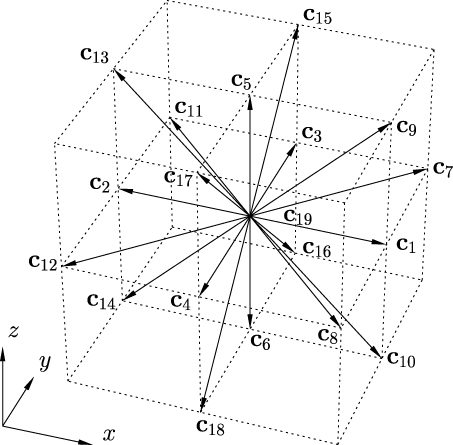
\includegraphics[width=\singleimagewidth]{chapters/figures/lbm/4193301.jpg}\label{fig:d3q19-lattice}
\end{figure}

The numbered direction in the lattice of Fig.~\ref{fig:d3q19-lattice} follows the standard practice of LBM. The index $i=0$ corresponds to the node center. The indices $i = 1,2,3,\dots,6$ point to the six faces of the cube surrounding the node. Lastly, the indices $i=7,8,9,\dots,18$ point to the twelve midpoints of the edges of the cube. The weight constants, satisfying lattice symmetry, of the lattice structure of Fig.~\ref{fig:d3q19-lattice} are calculated in Ref.~\cite{Latt2007} and given as,
\begin{equation}\label{eq:d3q19-weights}
	w_i = \begin{cases}
	\frac{1}{3}			& i = 0\\
	\frac{1}{18} 		& i = 1,2,3,\dots,6\\
	\frac{1}{36}		& i = 7,8,9,\dots,18
	\end{cases}
\end{equation}

The lattice weights, $w_i$ are necessary to account for the different vector lengths in the lattice. In principle, there is freedom in choosing the lattice speed of sound, $c_s$, requiring a change to the rest-weight of $w_0$ to maintain lattice symmetry. However, in practice, it is common to use $c_s^2 = \frac{1}{3}$ for numerical stability.\cite{Latt2007,succi2001lattice}.




\subsection{Boundary Conditions}
Implementation of no-slip boundary conditions at the wall in the lattice-Boltzmann method are direct descendants of the schemes from lattice gas automata: a bounce-back scheme. In the scheme, lattice nodes that at the boundary have particle directions that point into the wall. For example, see $f_4$, $f_7$, and $f_8$ in Fig.~\ref{fig:wall-lattice-bc}. In this configuration, as particles stream into the wall, their distributions are scattered back in equal and opposite directions. Computationally, the bounce-back scheme is very attractive for the simplicity of implementing the method even in complex geometries. A fact which makes the use in LBM particularly attractive for packed bed simulations.\cite{Chen1998a} The bounce-back scheme has been shown to be first-order accurate for most three-dimensional flows, degrading the other-wise second order accuracy of the fluid bulk calculations.\cite{Zou1997,Chen1998a} To combat the loss in accuracy, several modifications to the bounce-back scheme have been proposed (see Ref.~\cite{Chen1998a}). However, for the porous flow to be studied in ceramic pebble beds, it suffices to implement the bounce-back boundary condition to enforce no-slip.\cite{Chen1998a,Luo2003a}

\begin{figure}[t]
	\centering
	\caption{Sketch of the D2Q9 nodes; showing at the boundary the distribution functions that would come from neighbors outside the boundary (in the solid) are unknown (reproduced from Ref.~\cite{Parmigiani2011}).}
	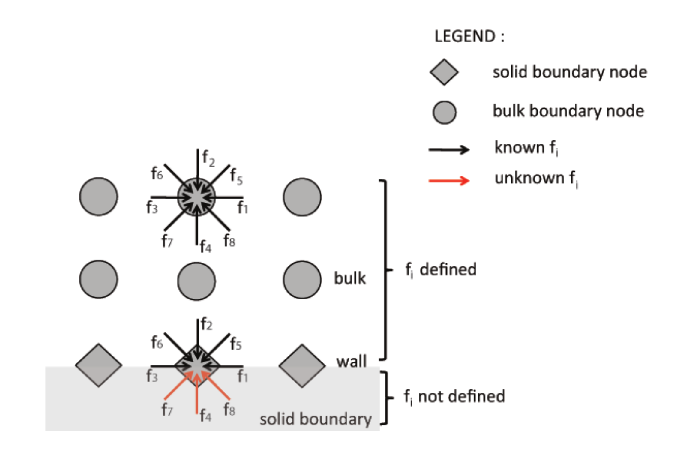
\includegraphics[width=\singleimagewidth]{chapters/figures/lbm/wall-lattice-bc}\label{fig:wall-lattice-bc}
\end{figure}


To treat velocity or pressure boundary conditions, we use the technique of Zou \& He.\cite{Zou1997} They proposed extending the bounce-back condition to the non-equilibrium distribution function in the direction normal to the boundary. The approach allows closure of the algebraic calculation of distribution functions when we have a known, physical, velocity or pressure (see Eqs.~\ref{eq:lbm2physical}). We note again that, in lattice units, determination of density is equivalent to determination of pressure via the ideal gas pressure law. Zou \& He showed the approach provides second-order accurate results.\cite{Zou1997} 












\subsection{Thermal LBM}

Thus far the lattice-Boltzmann formulation allows us to calculate mass and momentum transport of a fluid. But in the packed beds of fusion reactors, the transport of energy in the system is of utmost importance. To handle the thermal equations in the lattice-Boltzmann framework, we use the model of Guo\etal.\cite{Guo2002} Guo\etal~introduced a second lattice upon which the distribution functions for temperature resided. The temperature distribution evolved with a coupling to the velocity distribution on the lattice solving the Navier-Stokes equations. The temperature was linked back to the Navier-Stokes lattice with a Boussinesq assumption that introduced a body force term to the fluid.\cite{Guo2002} Guo\etal~referred to their approach at the Coupled Lattice BGK (CLBGK) method. 

On the thermal lattice in the CLBGK method, the temperature is a passive scalar that is transported by the velocity (it is specified at each node corresponding to the overlapped nodes from lattice solving the Navier-Stokes equations). Therefore, the density of the Navier-Stokes lattice is equivalent to the temperature on the thermal lattice. The thermal lattice BGK equation is analagous to Eq.~\ref{eq:lbm-bgk},
\begin{equation}\label{eq:lbm-thermal-bgk}
	T_i(\vec{x}+\vec{c}_i, t + 1) = T_i(\vec{x},t) - \frac{1}{\tau_T}\left[T_i^\eq(\vec{x},t) - T_i(\vec{x},t)\right]
\end{equation}
where we have a second relaxation time for the thermal lattice, $\tau_T$. The temperature field is reconstructed via
\begin{equation}
	T = \sum_i^q T_i
\end{equation}

A multi-scale expansion of Eq.~\ref{eq:lbm-thermal-bgk} can show that it is equivalent to the temperature form of the continuous energy conservation equation.\cite{Guo2002} For the transport of the passive scalar, we can use a D3Q7 lattice which is sufficient to model the advection-diffusion of temperature.\cite{Latt2007,Parmigiani2011}), For such a lattice, the speed of sound is $c^2_{s,ad} = \frac{1}{2}$. We use a linear equilibrium function for $T_i^\eq$,
\begin{equation}
	T_i^\eq = w_i T (1+\frac{\vec{c}_i\cdot\vec{u}}{c_s^2})
\end{equation}

The thermal diffusivity (analogous to the viscosity in the momentum lattice) is 
\begin{equation}
	\alpha_{lb} = c_{s,ad}^2(\tau_{ad} - \frac{1}{2})
\end{equation}
% The coupling from temperature to density via the Boussinesq assumption is done with the addition of a body force term, $g_i$ to the Navier-Stokes' BGK equation,
% \begin{equation}
% 	f_i^\eq = \rho(\vec{x},t)w_i\left[1+\frac{\vec{u}\cdot\vec{c}_i}{c_s^2} + \frac{(\vec{u}\cdot\vec{c}_i)^2}{2c_s^4} - \frac{\vec{u}^2}{2c_s^2} \right] + g_i
% \end{equation}
% where the body term is
% \begin{equation}
% 	g_i = -\frac{1}{2}\Delta t \alpha_i \vec{c}_i\cdot\vec{g}(T - T_0)
% \end{equation}

Thermal boundary conditions are handled via a decomposition of the boundary nodes into equilibrium and non-equilibrium parts and the values of the node extrapolated from neighboring nodes. Details of the precise equations can be found in the paper by Guo\etal.\cite{Guo2002}






\subsection{LBM for Porous Flow}
The lattice-Boltzmann technique, because of its incredibly simple implementation of no-slip boundary conditions for even the most complex geometry, was immediately seen as a powerful option of fluid modeling in porous networks. Chen \& Doolen review many of the major accomplishments of implementing LBM models which verified Darcy's Law, the Cozeny-Karman equation, and Brinkmann equation among other efforts.\cite{Chen1998a} Pan\etal~evaluated the single-relaxation time BGK operator against models with multiple relaxation times as well as the differences with implemented various fluid-solid interface boundary conditions -- among which was the bounce-back scheme we use here.\cite{Pan2006}